This kind of approach has not been attempted until now, so it is a novel way of handling data in a distributed environment, using \ac{sql}. There has been some development on the subject using other query languages as \ac{cql}, as for distributed transactions the studies mostly address the problem using some kind of leader. 


\section{\acl{cql}}

The \ac{cql} \cite{cql}, is a really novel approach to this matter, being developed by Eric Evans. His idea, is to develop a \ac{sql} like query language on top of Cassandra, bypassing an \ac{sql} interpreter altogether at the expense of not being compatible with actual \ac{sql}  code. Still, this would allow for much faster adaptation to Cassandra, for people with relational background. 

\ac{cql} has been released with Cassandra new stable version (0.8), and a select query will look somewhat like this \cite{cqlSelect}:

\begin{center}
\begin{verbatim}
    SELECT (FROM)? <CF> [USING CONSISTENCY.<LVL>] WHERE 
       <EXPRESSION> [ROWLIMIT X] [COLLIMIT Y] [ASC|DESC]
\end{verbatim}
\end{center}

And would be replacing a lot of old methods for retrieving data as \emph{get()}, \emph{get\_slice()}, \emph{get\_range\_slices()}, and so on.	

At the time of writing there are still some features to be implemented\cite{cqlbbw}, such as \emph{ALTER} and prepared statements and some SQL features that will not be implemented at all, as joins and update\footnote{Since cassandra 0.7 the updates are viewed as a special case of insert}.

\section{Distributed Transactions}

Transactions become difficult under heavy load. When you first attempt to horizontally scale a relational database, making it distributed, you must now account for distributed transactions, where the transaction isn’t simply operating inside a single table or a single database, but is spread across multiple systems. In order to continue to honor the ACID properties of transactions, you need a transaction manager to orchestrate across the multiple nodes.

There are many leader election algorithms but they all have the same input and output. At the beginning there is a set of nodes in a network, unaware of which of them is the leader, after the protocol they all recognize a particular, unique node as the leader.

Assuming that the leader is already elected, a simple way to complete a distributed transaction in an atomic manner is for the coordinator to communicate the commit or abort request to all of the participants in the transaction and keep repeating the request until all of them have acknowledged that they have carried it out. This is called one-phase commit protocol\cite{coulouris2005distributed} and is inadequate because it does not allow a server to make a unilateral decision to abort a transaction. 

\subsection{Two-phase commit protocol}

The two-phase commit protocol is designed to allow any participant to abort its part of a transaction which, by the atomicity requirement, means the whole transaction must be aborted. 

In the first phase of the protocol the coordinator asks all of the participants if they are prepared to commit and in the second it tells them to commit/abort the transaction. Once a participant has voted to commit a transaction it is not allowed to abort it, therefore a participant must before make sure it will be able to carry out its part of the protocol, before committing to it. 

\begin{table}[h!]
\centering
  \begin{tabular}{  l | p{8cm}}
	Operation & Description\\
    \hline  \hline
    \emph{canCommit?(trans) $\rightarrow$ Yes/No} & Coordinator asks if it can commit a transaction. Participant replies with vote.\\
    \hline
    \emph{doCommit(trans)} & Coordinator tells participant to commit its part.\\
    \hline
    \emph{doAbort(trans)} & Coordinator tells participant to abort its part.\\
    \hline
    \emph{haveCommited(trans,participant)} & Participant asks the coordinator to confirm it has commited.\\
    \hline
    \emph{getDecision(trans) $\rightarrow$ Yes/No} & Participant asks for decision after it has voted. Used to recover from server crashes or delayed messages.
  \end{tabular}

\caption{Operations for two-phase commit protocol (based on \cite{coulouris2005distributed})}
\label{tab:2pc_ops}
\end{table}

Using the operations defined in table \ref{tab:2pc_ops}, a successful run of the protocol with one coordinator and one participant is as shown by figure \ref{fig:2pc_run}.

\begin{figure}[htb]
  \begin{center}
    \leavevmode
    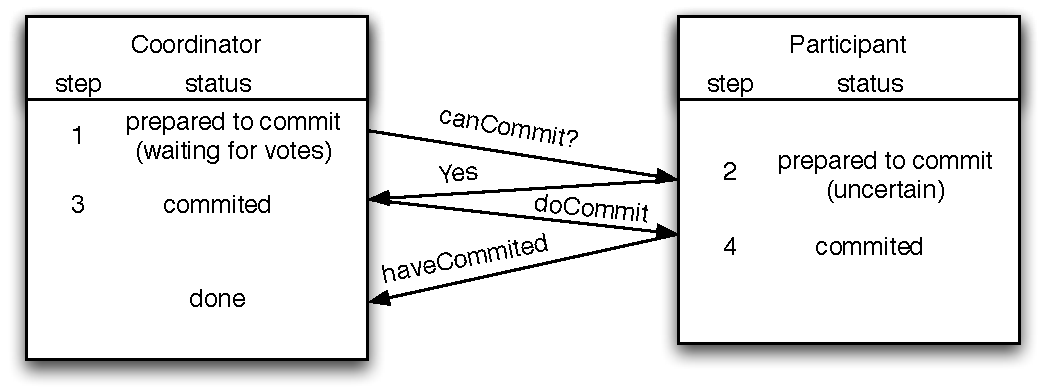
\includegraphics[width=0.9\textwidth]{images/2pc}
  \end{center}
  \caption{Two-phase commit successful run\cite{coulouris2005distributed}}
  \label{fig:2pc_run}
\end{figure}

\subsection{Three-phase commit protocol}

\section{\emph{Sharding}}

Another way to attempt to scale a relational database is to introduce \emph{sharding} to your architecture. The idea is to split the data across multiple machines in such a way that when clients executes queries they put the load in only one machine. From this definition comes that in order to shard you need to find a good key to order the records. There are three basic strategies for determining shard structure:

\begin{description}
	\item[Feature-based shard]  Using this strategy, the data is split not by dividing records in a single table, but rather by splitting into separate databases the features that do not overlap with each other very much. This approach depends on understanding your domain so that you can segment data cleanly.
	\item[Key-based \emph{sharding}] In this approach, you find a key in your data that will evenly distribute it across shards such as a one-way hash. It is common in this strategy to find time-based or numeric keys to hash on.
	\item[Lookup table] In this approach, one of the nodes in the cluster is responsible for looking up which node has the data you are trying to access. This has two obvious disadvantages. The first is the lowering in performance every time you have to go through the lookup table as an additional hop. The second is that the lookup table not only becomes a bottleneck, but a single point of failure.
\end{description}

\emph{Sharding} relates to shared nothing architecture\cite{University86thecase}\footnote{A shared-nothing architecture is one in which there is no centralized (shared) state, but each node in a distributed system is independent, so there is no client contention for shared resources.} in the sense that once \emph{sharded}, each shard lives in a totally separate logical schema and physical server. This is the same overall architecture as BigTable and Cassandra from which comes that both are used to scale databases horizontally, and therefore encounters some of the same issues. For example, the auto-increment key system that is so widely used for primary keys, generates a sequential key for each row inserted, which is fine for a single database application, but with \emph{sharding} there is a need for a centralized manager that ensures that the keys are unique across the entire system.
